\documentclass{beamer}
\usepackage[T2A]{fontenc}
\usepackage[utf8]{inputenc}
\usepackage[russian]{babel}
\mode<presentation> {
\usetheme{Madrid}
}

\usepackage{tikz}
\usetikzlibrary{positioning}
\usetikzlibrary{circuits}
\usetikzlibrary{circuits.ee}
\usetikzlibrary{circuits.ee.IEC}
\usetikzlibrary{circuits.logic.IEC}

\usepackage{graphicx}

\usepackage[russian]{babel}

\uselanguage{Russian}
\languagepath{Russian}

\newtheorem{proposition}[theorem]{\translate{Теорема}}

%----------------------------------------------------------------------------------------
%	TITLE PAGE
%----------------------------------------------------------------------------------------

\title[Оценка области захвата для систем]{Оценка области захвата для систем ФАПЧ 3 порядка} % The short title appears at the bottom of every slide, the full title is only on the title page

\author{Миронов Алексей Владиславович} % Your name
\institute[СПБГУ] % Your institution as it will appear on the bottom of every slide, may be shorthand to save space
{
Санкт-Петербургский государственный университет\\ % Your institution for the title page
\vspace{0.7cm}
    Научный руководитель:  д.ф.-м. н., профессор Юлдашев Р. В. \\
    \vspace{0.7cm}
}
\date{\today} % Date, can be changed to a custom date

\begin{document}

\begin{frame}
\titlepage % Print the title page as the first slide
\end{frame}

%----------------------------------------------------------------------------------------
%	PRESENTATION SLIDES
%----------------------------------------------------------------------------------------

\begin{frame}
\frametitle{Принцип работы ФАПЧ}
\begin{definition}
Система фазовой автоподстройки частоты (ФАПЧ) - система предназначенная для синхронизации частот эталонного и подстраиваемого генераторов
\end{definition}
Применение системы ФАПЧ
\begin{enumerate}
\item Телекоммуникационное обородование
\item Навигационное оборудование (GPS, Глонасс, Галилео)
\item Компьютеры (микропроцессоры)
\end{enumerate}
\end{frame}

\begin{frame}
\frametitle{Принцип работы ФАПЧ}
\begin{center}
\resizebox{0.8\columnwidth}{!}{%
\begin{tikzpicture}
\node at (2,0) [draw, text width=4cm, align=center, rectangle] (a) {Фазовый детектор \par(компаратор)};
\node[draw, align=center, rectangle] (loop_filter) [right=of a] {Фильтр};
\node[draw, align=center, rectangle] (VCO) [right=of loop_filter] {ГУН};

\draw[->] (-3,0) -- (a.west);
\draw[->] (a.east) -- (loop_filter.west);
\draw[->] (loop_filter.east) -- (VCO.west);
\draw[->] (VCO.east) -- (11,0);
\draw[->] (10,0) --  +(0,-2) --  +(-8,-2) --  (a.south);

\end{tikzpicture}
}
\end{center}

Система дифференциальных уравнений описывающих работу ФАПЧ
 \begin{equation}\label{pllequations}
 \begin{aligned}
 &\dot{x} = Ax + b\upsilon_e(\theta_e) \\
 &\dot{\theta}_e = \omega_e^{free} - K_{vco}(c^*x + h\upsilon_e(\theta_e))
 \end{aligned}
\end{equation}
В системе \eqref{pllequations} сделаем следующие преобразования $-K_{vco}c \rightarrow c$, $-K_{vco}h \rightarrow h$ и замену
 \begin{equation}
 \begin{aligned}
 z = x + A^{-1}b\gamma  \text{,} \quad \gamma = \frac{\omega_e^{free}}{c^*A^{-1}b-h}
 \end{aligned}
\end{equation}
В результате \eqref{pllequations} примет вид
 \begin{equation}\label{system}
 \begin{aligned}
 &\dot{z} = Az + b(\upsilon_e(\theta_e) - \gamma) \\
 & \dot{\theta_e} = c^*z + h(\upsilon_e(\theta_e) - \gamma))
 \end{aligned}
\end{equation}
\end{frame}

\begin{frame}
Рассмотрим систему \eqref{system}
 \begin{equation*}
 \begin{aligned}
 &\dot{z} = Az + b(\upsilon_e(\theta_e) - \gamma) \text{,} \quad \dot{\theta_e} = c^*z + h(\upsilon_e(\theta_e) - \gamma))
 \end{aligned}
\end{equation*}
Пусть $\upsilon_e(\theta_e)$ дифференцируема на $\mathbb {R}$ и удовлетворяет $\mu_1 \leq \frac{d\upsilon_e(\theta_e)}{d\theta_e} \leq \mu_2$
 \begin{equation}
 \begin{aligned}
\nu = \int_{0}^{2\pi} (\upsilon_e(\theta_e) - \gamma) d\theta_e \left(\int_{0}^{2\pi} \mid \upsilon_e(\theta_e) - \gamma \mid d\theta_e\right)^{-1}
 \end{aligned}
\end{equation}
\begin{theorem}
Пусть все нули функции $\upsilon_e(\theta_e) - \gamma$ изолированы, пара $(A, b)$ вполне управляема, все собственные значения матрицы $A$ имеют отрицательные вещественные части и существуют числа $\varepsilon > 0, \delta > 0, \tau \geq 0$, и $\varkappa$, такие что имеют место неравенства:
 \begin{align}
&Re(\varkappa K(ix)- \varepsilon(K(ix))^2-[K(ix)+\mu_1^{-1}ix]^*\tau[K(ix)+\mu_2^{-1}ix])\geq\delta\text{,}\forall x \in \mathbb{R}\label{first_th_eq}\\
&4\varepsilon\delta > (\varkappa\nu)^2
\end{align}
Тогда система \eqref{system} глобально ассимптотически устойчива.
\end{theorem}
\end{frame}

\begin{frame}
\frametitle{Постановка задачи}
Оценить полосу захвата для систем, описывающихся следующими передаточными функциями:
 \begin{equation*}
 \begin{aligned}
&F(s) = \frac{1}{(1+\tau_{p1}s)(1+\tau_{p2}s)}\\
&\\
&F(s) = \frac{(1+\tau_{z1}s)^2}{(1+\tau_{p1}s)^2}\\
&\\
&F(s) = \frac{(1+\tau_{z1}s)(1+\tau_{z2}s)}{(1+\tau_{p1}s)(1+\tau_{p2}s)}
 \end{aligned}
\end{equation*}
\end{frame}

%------------------------------------------------

\begin{frame}
\frametitle{Фильтр $F(s) = \frac{1}{(1+\tau_{p1}s)(1+\tau_{p2}s)}$}
Оценка параметра $\nu^2$ для фильтра $F(s) = \frac{1}{(1+\tau_{p1}s)(1+\tau_{p2}s)}$
\begin{equation*}
\frac{(\tau_{p1}\tau_{p2} - 1)^2}{\tau_{p1}^2 + \tau_{p2}^2 + 1} > \nu^2
\end{equation*} 
\begin{columns}[onlytextwidth]
\begin{column}{.45\textwidth}
\begin{figure}
  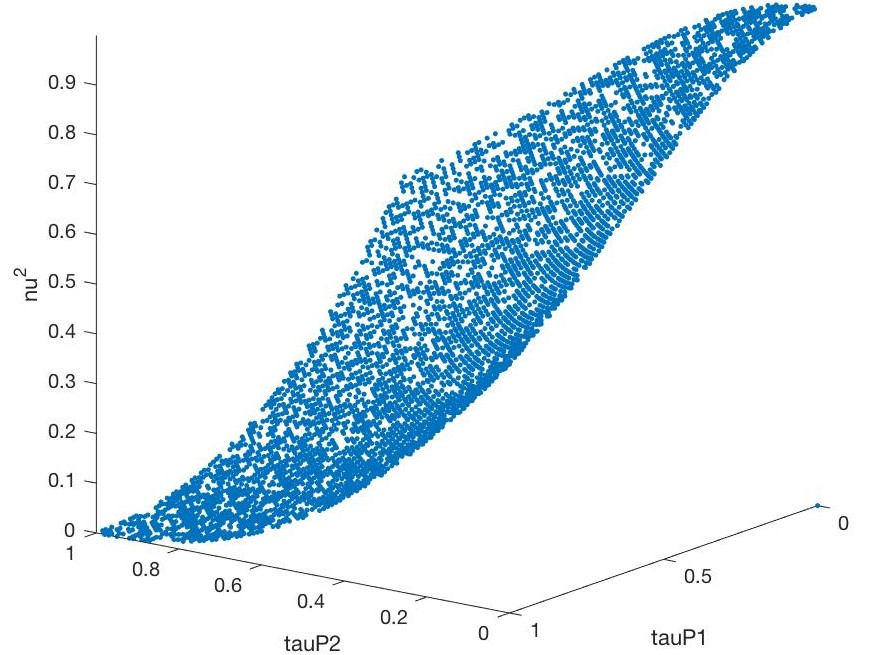
\includegraphics[width=\textwidth]{images/filter1e.jpg}
  \caption{First image}
\end{figure}
\end{column}
\hfill
\begin{column}{.45\textwidth}
\begin{figure}
  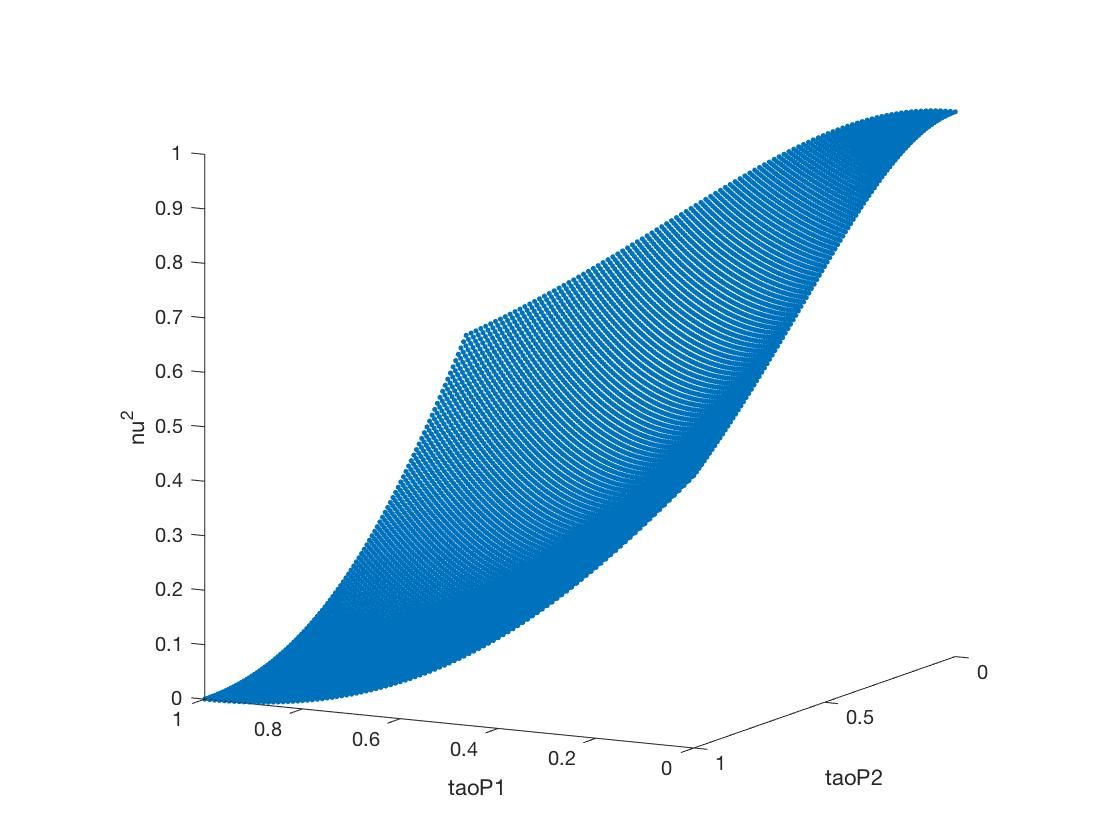
\includegraphics[width=\textwidth]{images/filter1_1.jpg}
  \caption{Second image}
\end{figure}
\end{column}
\end{columns}
\end{frame}

%------------------------------------------------

\begin{frame}
\frametitle{Фильтр $F(s) = \frac{(1+\tau_{z1}s)^2}{(1+\tau_{p1}s)^2}$}

Оценка параметра $\nu^2$ для фильтра $F(s) = \frac{(1+\tau_{z1}s)^2}{(1+\tau_{p1}s)^2}$
  \begin{figure}[H]
  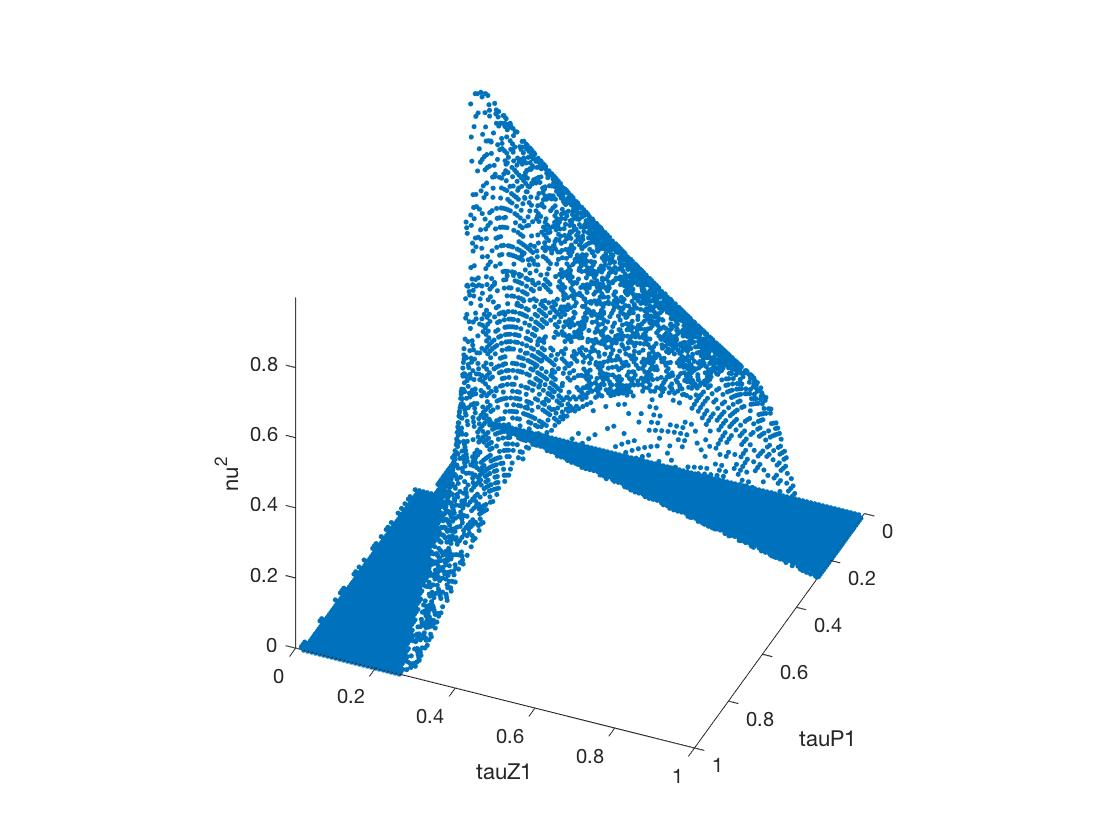
\includegraphics[width=5.7cm]{images/filter2_tau0_1e.jpg}
  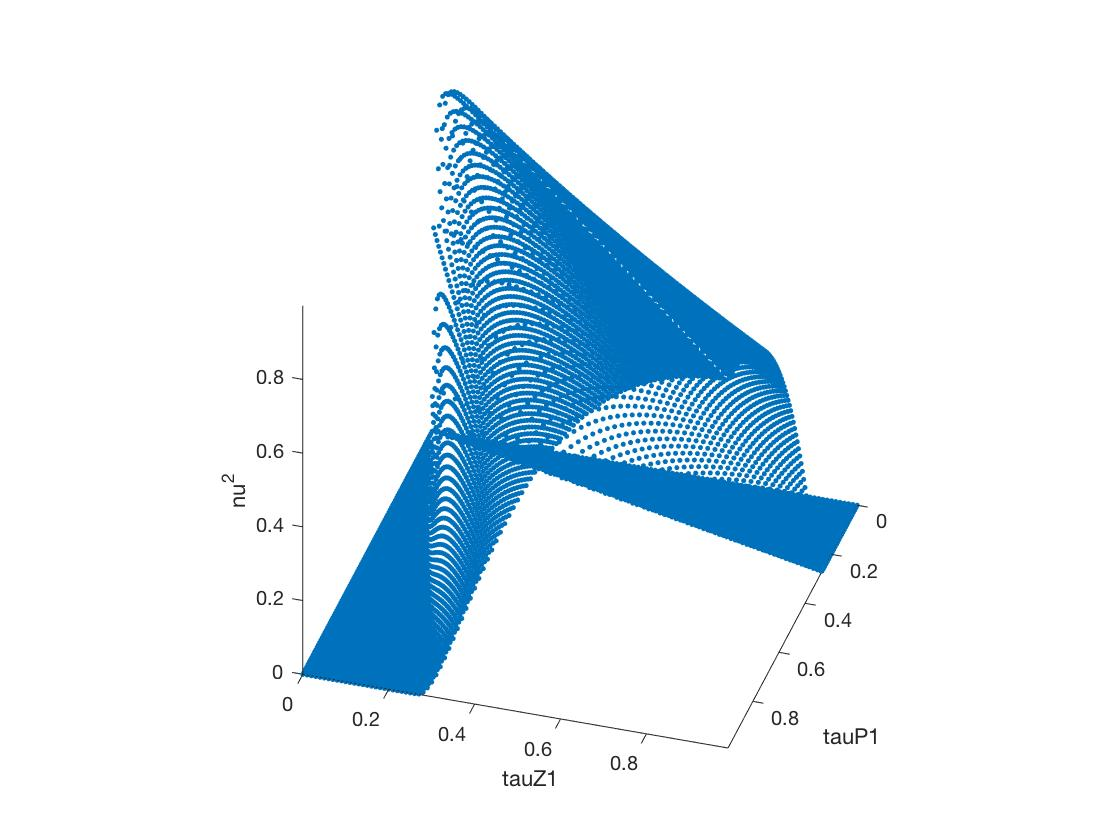
\includegraphics[width=5.7cm]{images/filter2_tau0_1.jpg}
    \caption{1. Численное приближение в MATLAB 2. Аналитическое решение}
    \end{figure}

\end{frame}

\begin{frame}
\frametitle{Фильтр $F(s) = \frac{(1+\tau_{z1}s)^2}{(1+\tau_{p1}s)^2}$}

  \begin{figure}[H] 
  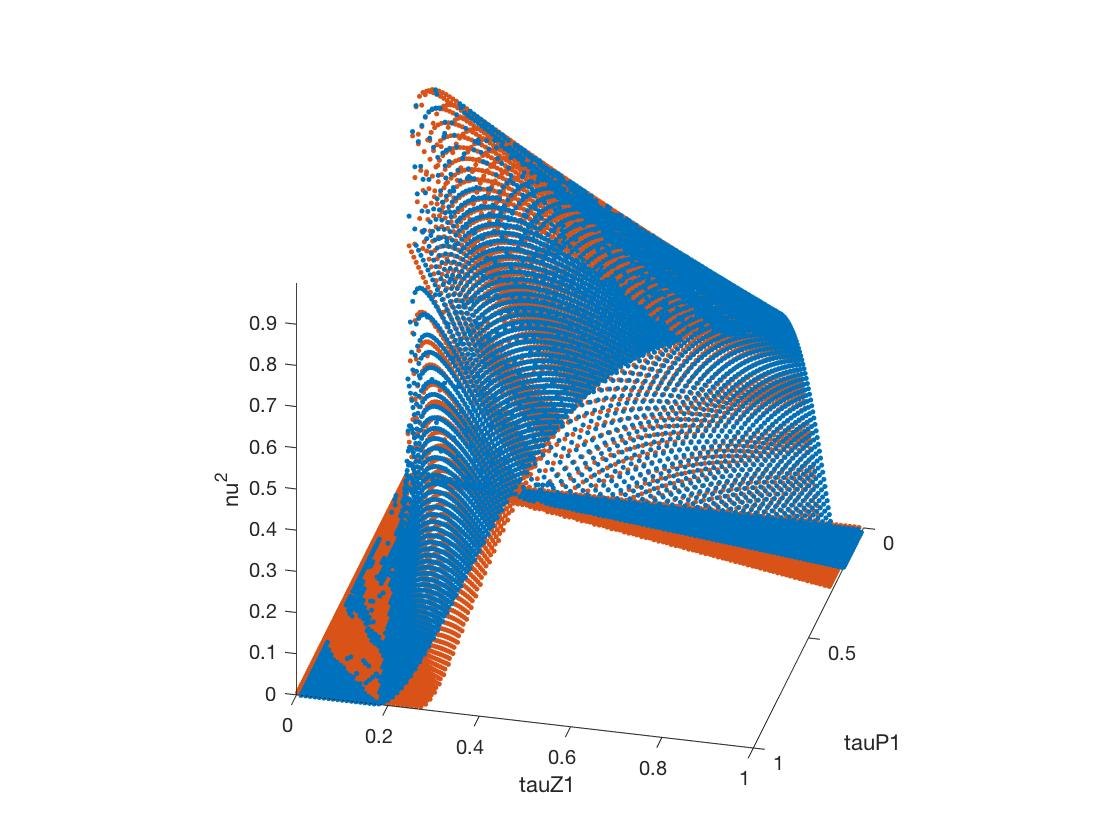
\includegraphics[width=7cm]{images/main.jpg}
\caption{График зависимости $\nu^2$ от $\tau_{p1}, \tau_{p2}$.  Синим цветом представлено точное решение. Оранжевым цветом представлено аналитическое решение.}
\end{figure}

\end{frame}

%------------------------------------------------

\begin{frame}
\frametitle{Фильтр $F(s) = \frac{(1+\tau_{z1}s)(1+\tau_{z2}s)}{(1+\tau_{p1}s)(1+\tau_{p2}s)}$}
При рассмотрении фильтра $F(s) = \frac{(1+\tau_{z1}s)(1+\tau_{z2}s)}{(1+\tau_{p1}s)(1+\tau_{p2}s)}$  получаем следующую оценку параметра $\nu^2$:
 \begin{equation*}
 \begin{aligned}
&\nu^2 < 4\frac{[\alpha_1^2(1-\beta_1) - \alpha_2(1-\beta_2)][\alpha_1^2(1-\beta_1)\beta_1 - \alpha_2(1-\beta_2)]}{[\alpha_1^2(1-\beta_1^2) - 2\alpha_2(1-\beta_2)]^2}\\
&\alpha_1 = \tau_{p1} + \tau_{p2}\text{,}\quad 
\alpha_2 = \tau_{p1}\tau_{p2}\text{,}\quad 
\beta_1 = \frac{\tau_{z1}+\tau_{z2}}{\tau_{p1}+\tau_{p2}}\text{,}\quad 
\beta_2 = \frac{\tau_{z1}\tau_{z2}}{\tau_{p1}\tau_{p2}}
 \end{aligned}
\end{equation*}
\end{frame}

%------------------------------------------------

\begin{frame}
\Huge{\centerline{Спасибо за внимание}}
\end{frame}

%----------------------------------------------------------------------------------------

\end{document} 